\section{Experimental Evaluation} % 70/300 points, 23%

We fine-tune and evaluate the \BertSumAbs summarization model from the reproduced paper by \citeauthor{LiuL2019} on a A100 GPU using the Flux framework on Julia~\cite{InnesSFGRJKPS2018,BezansonEKS2017,LiuL2019}.
A scaled-down variant of their \TransformerAbs model, that we call \TransformerAbsTiny, is trained from scratch on a GeForce MX150 GPU for testing our evaluation workflow.
We train both models using the CNN/Daily Mail datasets, but use the preprocessed variant by \citeauthor{LiuL2019} instead of the original data by \citeauthor{HermannKGEKSB2015}~\cite{LiuL2019,HermannKGEKSB2015}.
Our implementation resembles the same encoder-decoder architecture as used by \citeauthor{LiuL2019}, uses the same \BertBase model for the pretrained encoder, and \Bert's WordPiece tokenizer to transform raw text into tokens that can be embedded~\cite{LiuL2019,DevlinCLT2019}.
Though, we do not tune any hyperparameters of either the model or the optimizers.
We also reimplement the beam search algorithm from scratch.
Due to instabilities in fine-tuning and hardware constraints we were unable to train the model for the full 200\,000 steps proposed by \citeauthor{LiuL2019}~\cite{LiuL2019}.
We assume that the complex hyperparameter settings and large model size used in their paper are prone to fine-tuning issues like we experienced, a problem that has only recently gained more attention~\cite{DodgeISFHS2020,ZhangWKWA2020,AghajanyanSGGZG2020}.

\subsection{Dataset}

We train and evaluate the summarization model on the CNN/Daily Mail benchmark dataset using the standard training, test, and validation splits, as crawled by \citeauthor{NallapatiZSGX2016}~\cite{HermannKGEKSB2015,NallapatiZSGX2016}.
\citeauthor{LiuL2019} preprocess the raw non-anomized CNN/Daily Mail dataset, split sentences with the Stanford CoreNLP framework~\cite{ManningSBFBM2014}, and release the preprocessed data publicly~\cite{LiuL2019}.
Our implementation is designed to automatically download those preprocessed CNN/Daily Mail datasets from the Web\footnote{\url{https://drive.google.com/open?id=1DN7ClZCCXsk2KegmC6t4ClBwtAf5galI}}, no manual downloads are needed.

Even though \citeauthor{LiuL2019} claim to truncate input sequences after 512 tokens, we observe sequences longer than 512 tokens in the preprocessed data~\cite{LiuL2019}.
We use the opportunity to not truncate input sequences, as truncating after only 512 discards a reasonable amount~(33\,\% on average) of context from a news article~\cite{NallapatiZSGX2016}.\footnote{It could be reasoned that especially the last sentences of an article be relevant for drawing the right conclusion in a summary.}
From the preprocessed data we extract pairs of each source article with its target summary, normalize sentence separators, and tokenize with \Bert's WordPiece tokenizer~\cite{DevlinCLT2019}.

Like \citeauthor{LiuL2019}, we use the \BertBase model, pretrained by \citeauthor{DevlinCLT2019}, as encoder~\cite{DevlinCLT2019}.
That \Bert model is also automtically downloaded from the Web along with its WordPiece tokenizer.\footnote{\BertBase is loaded using the Transformers Julia library: \url{https://github.com/chengchingwen/Transformers.jl}}

\subsection{Abstractive Summarizaion Model}

Transformer with 6 layers, 768 hidden units, hidden size of 2048.
Train for 200\,000 steps, snapshots every 2500 steps, gradient accumulation at every step.
Choose the single best snapshot for evaluation.

Describe simple tests/examples for checking implementation correctness. (Untrained model produces nonsense summaries.)

Describe implementation memory usage, complexity, and run time performance.
The full \BertSumAbs model contains 182M trainable parameters: 27M for embeddings, 85M for the encoder's transformer layers, 47M for the decoder's transformer layers, and 23M for the generator layer.

\subsection{Fine-tuning the pretrained model}

Describe training schedule.
Two Adam optimizers with~\(\beta_1 = 0.9\) and~\(\beta_2 = 0.999\).
Learning rates:
\begin{align}
    \eta_E &= 2e^{-3} \cdot \min( \text{step}^{-0.5},\ \text{step} \cdot 20\,000^{-1.5} ) \\
    \eta_D &= 0.1 \cdot \min( \text{step}^{-0.5},\ \text{step} \cdot 10\,000^{-1.5} )
\end{align}

Presumably because of the high number of parameters to tune, training this \BertSumAbs model on a A100 GPU uses about 40GB of memory at a speed of about 9 steps per minute.
Because of the slow training speed even on a powerful GPU we had to cancel training the model after 22\,500 steps.

\subsection{Beam Search}

\subsection{Experiments}

Describe experiment reproductions.

\paragraph{Training Loss}

\begin{figure}
    \centering
    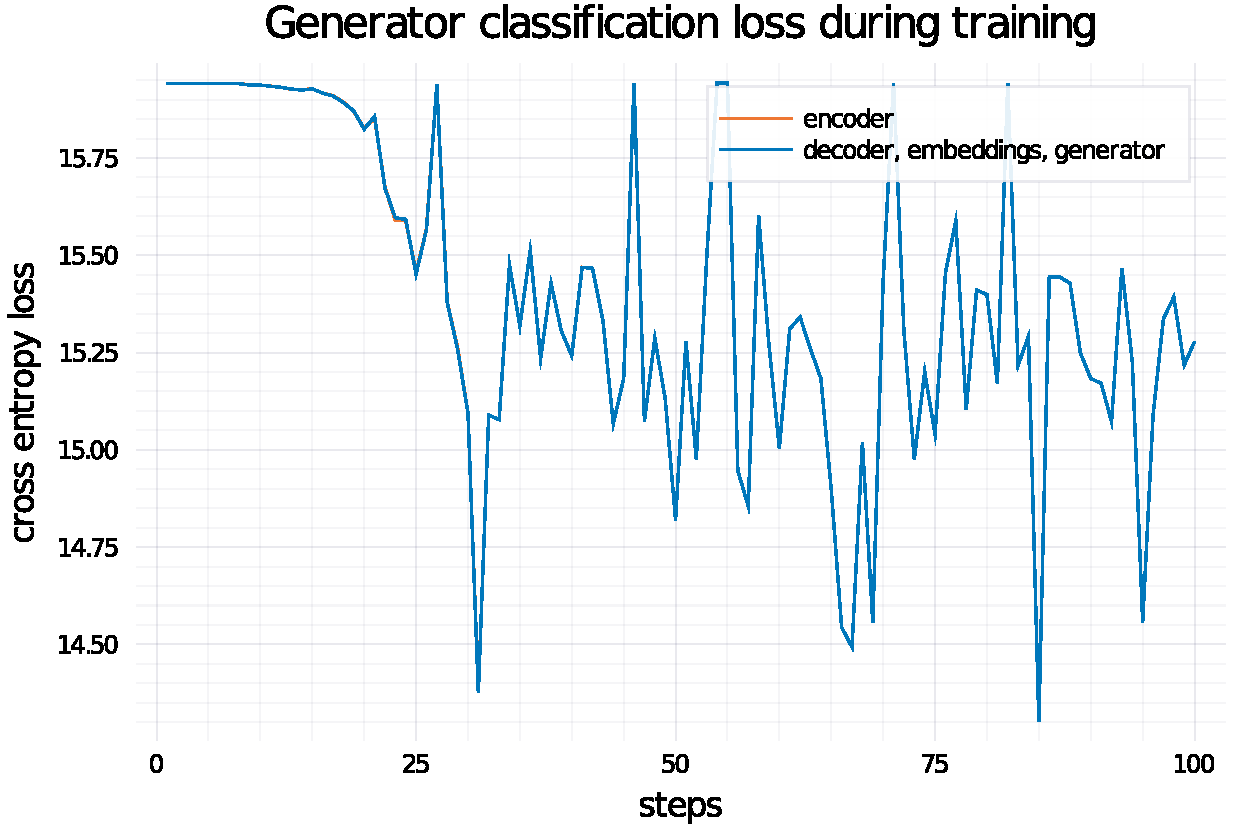
\includegraphics[width=0.7\linewidth]{training-loss-bert-abs-100.pdf}
    \caption{Cross entropy between predicted token probabilities and ground truth labels for the first 100 training steps of training the \BertSumAbs model.}
    \label{training-loss-bert-abs}
\end{figure}

\begin{figure}
    \centering
    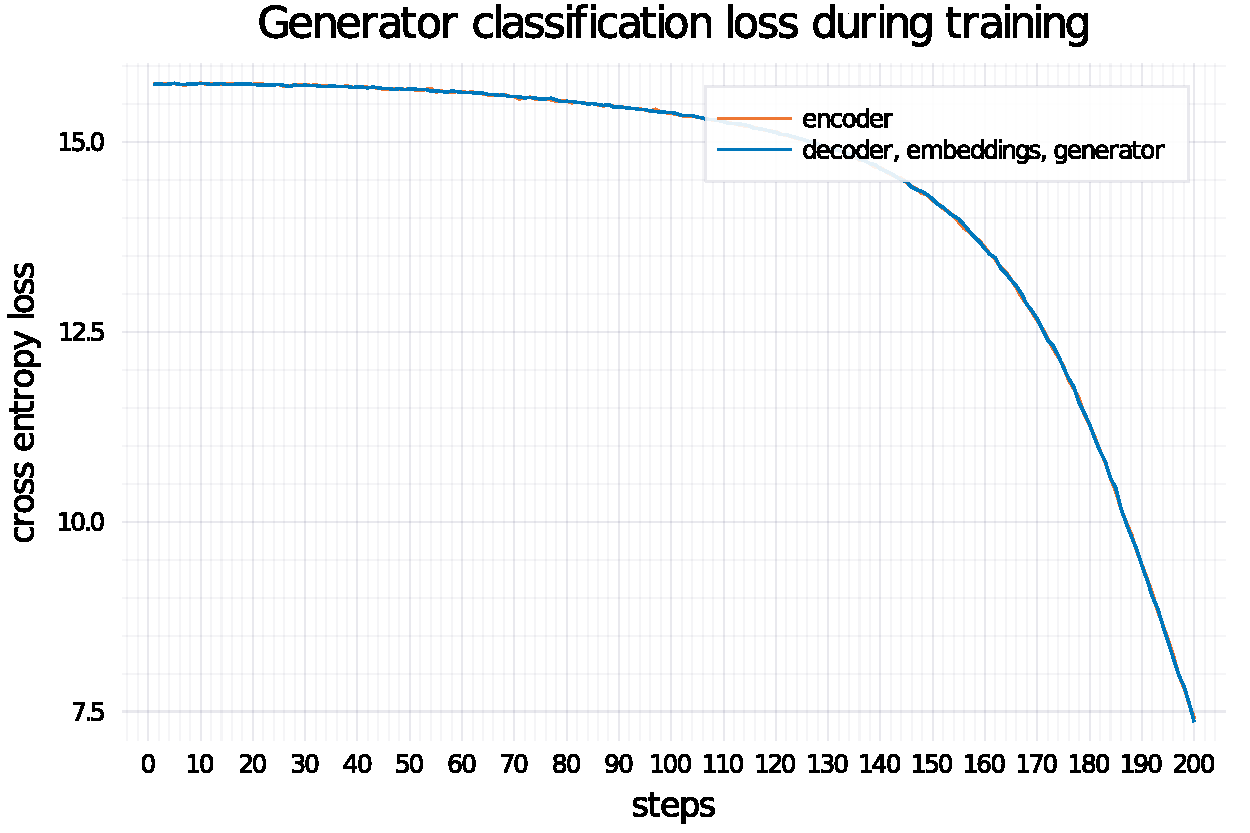
\includegraphics[width=0.7\linewidth]{training-loss-transformer-abs-tiny.pdf}
    \caption{Cross entropy between predicted token probabilities and ground truth labels for the first 200 training steps of training the \TransformerAbsTiny model.}
    \label{training-loss-transformer-abs}
\end{figure}


\paragraph{Summary Quality}

Describe \Rouge scores for some examples.

Describe/list difficulties or problems. (Pretrained data not available from a data source that allows automatic downloads.)
